\section{Optimization}

\subsection{Hybrid CORDAC}
\begin{frame}
    \frametitle{Hybrid CORDAC}
		Cache-efficient algorithm recursive subdivision continues until 
		the problem size becomes small enough.
	\begin{itemize}
		\item Benefits of both iterative and recursive algorithms
		\item Asymptotic improvement in parallelism
		\item Highly optimizable base cases
	\end{itemize}
\end{frame}

\subsection{Optimizing Kernel Functions}
\begin{frame}
    \frametitle{Optimizing Kernel Functions}
	\begin{description}
		\item[Copy-optimization] Copy the data into local $b \times b$ 
			static arrays inside the kernel.
		\item[Loop Reordering] In flexible kernels, it is possible to change
			the looping order without hampering the correctness of the algorithm.
	\end{description}
\end{frame}

\subsection{Data Layout}
\begin{frame}
    \frametitle{Data Layout}
	\begin{figure}
		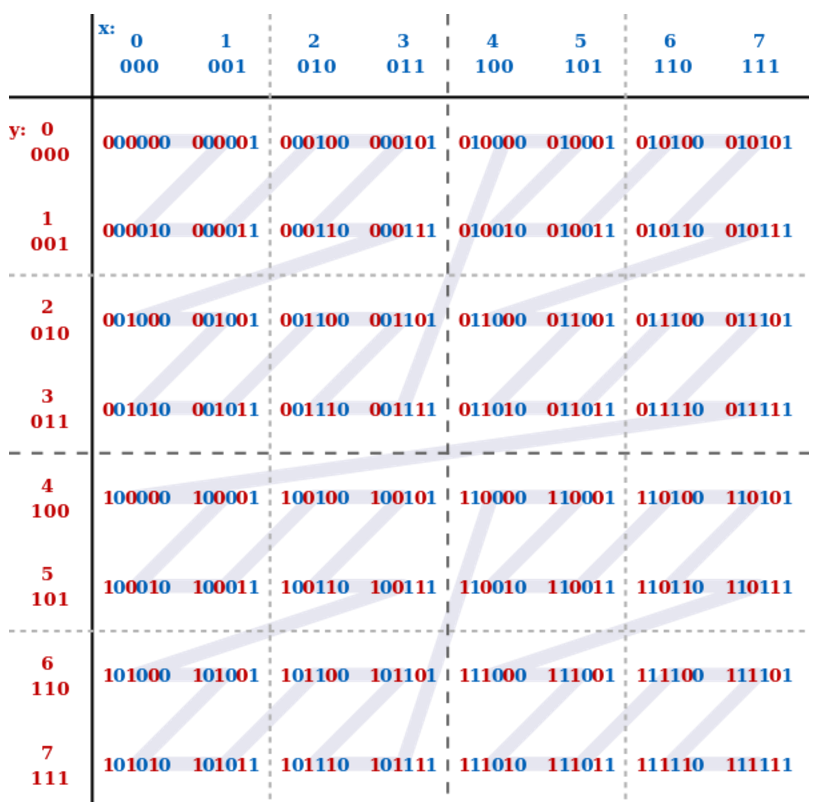
\includegraphics[scale=0.2]{figure/fig-z-morton.png}
	\end{figure}
	\begin{itemize}
		\item \textit{Z-Morton Row-Major}(ZM\_RM) layout is beneficial because
			it improves both temporal and spatial localities.
	\end{itemize}
\end{frame}

\subsection{Auto vs. Explicit Vectorization}
\begin{frame}
    \frametitle{Auto vs. Explicit Vectorization}
    It often vectorize the base-case of the dominating kernel.
	\begin{itemize}
		\item For example, $C_{\textit{loop}}$ is enough to get the 
			major share of the speedup.
	\end{itemize}
\end{frame}